\documentclass[12pt, class=article, crop=false]{standalone}
\usepackage[subpreambles=true]{standalone}
\usepackage[T1]{fontenc} % for font setting
\usepackage{tgtermes} % for font setting
\usepackage{import,
            graphicx,
            parskip,
            url,
            amsmath,
            wrapfig,
            soul}
\usepackage[most]{tcolorbox}
\usepackage[includeheadfoot,
            top=2.54cm,
            bottom=2.54cm,
            left=2.54cm,
            right=2.54cm]{geometry}%set margin
\usepackage[sort&compress]{natbib}
\setcitestyle{square}
\setcitestyle{comma}
\usepackage[font={sf, small}, labelfont={bf, small}]{caption}
\usepackage{fancyhdr}

\tcbuselibrary{breakable}
\bibliographystyle{bibstyle}

\begin{document}

\textbf{Research Strategy}

\section{Significance}

\subsection*{Background}

Over the past century, biologists have been intrigued by how interacting organisms are assembled in a given environment.
This process, termed ``community assembly,'' has crucial implications for human society's public health and sustainability.
For example, the community structure of human gut microbes impacts the development of the host immune system and protection against pathogen invasion.
Community assembly also plays a critical role in large-scale biological outcomes, such as the environmental restoration of degraded habitats in human-dominated landscapes.
The effect of environmental restoration on ecological communities is contingent on how colonizing species reach the restored site, often defining the ``success'' of the restoration project that managers invest millions of dollars for implementation.
Therefore, understanding the regulatory rules in community assembly (hereafter, ``assembly rule'') is fundamental to a broad range of biological phenomena.

The prevailing paradigm in community assembly suggests that the interaction between the environment and species attributes determines the structure of biological communities  (e.g., the relative abundance of different species) -- if the same set of species colonizes into a given habitat, the community structure will ultimately reach the identical state of community structure at equilibrium (the ``niche'' paradigm).
However, biologists have begun to recognize that, in certain circumstances, community dynamics are highly sensitive to the order of species colonization, leading to the divergent equilibrium state of the community structure despite the identical source of colonizing species and the environment.
This historical contingency of community state is referred to as ``priority effects,'' and their stochastic nature posed a significant challenge in predicting and maintaining community structure by conditioning the environment.
For example, it is often observed that the gut microbiome deviates far from the favorable state even if its ideal environment is maintained \textit{via} treatment.

The consequences of priority effects are well understood. Yet, a critical question remains unsolved: \ul{``\textit{when do priority effects occur?}}'' 
Answering this question is not only critical to advancing basic science but also helps solve issues concerning public health and the sustainability of natural resources.

\subsection*{Problem Statement}

The experimental manipulation of species' colonization order has been a common method -- perhaps \textit{the} method -- to confirm their existence; when priority effects manifest, the different colonization order of species leads to the divergent community states at the end of the experiment.
Over the past few decades, the results of the controlled experiments suggested the pervasiveness of priority effects across a wide variety of biological communities, including microbes, plants, and animals.
Even more, they spawned several influential hypotheses predicting the likely biological scenarios in which priority effects should matter.
For example, priority effects are hypothesized to be prevalent in the environment that enhances the rapid establishment of early colonizing species, such as small habitat size, high productivity, and low environmental variability, among others.

Nonetheless, some experts remain concerned about the prevalence and importance of priority effects because they have rarely been confirmed \textit{in unmanipulated natural systems}.
Often, controlled experiments are too small in scale and too simplified to be meaningful in the real world.
But, in natural systems, knowing the order of species' arrival is virtually impossible.
As such, resolving this fundamental problem requires a statistical method that captures the signature of priority effects \textit{without knowing the colonization history}.
We are unaware of such a novel statistical method, however. 

\subsection*{Solution}

\ul{We propose to fill this knowledge gap by developing a new statistical method that identifies biological communities sensitive to priority effects}.
Our method is motivated by the fact that time series data may provide deep insights into assembly rules.
In theory, assembly rules are set by the composition of species' traits within a given community, which dictates characteristic patterns of temporal community dynamics.
If niche-structured, species' niche differences produce the predominance of negative frequency dependence (= rarer species have greater population growth) such that rarer species can grow from small populations.
In contrast, when priority effects manifest, the positive frequency dependency of population growth (= dominant species have greater population growth) facilitates the stochastic dominance of a subset of species.
Our method will capitalize on these characteristic dynamics of distinct assembly rules to detect a signature of priority effects from a short time series.
To this end, our proposal is structured as follows:

\begin{itemize}
    \item \textbf{Specific Aim 1}: We will derive a theoretical backbone of this novel method.
    \item \textbf{Specific Aim 2}: We will assess the performance of the developed method using experimental biological communities, in which the order of species' arrival is manipulated.
    \item \textbf{Specific Aim 3}: We will apply the developed method to accumulating global time series data of biological communities. In doing so, we will ask: ``\textit{When are priority effects more likely to occur in natural systems?}''
\end{itemize}

\subsection*{Innovation}
Understanding assembly rules has far-reaching implications for human society's sustainability as it relates to human health, food production, and biodiversity conservation, to name just a few.
We assert that our proposal will advance this research field significantly through three important breakthroughs.
First, \ul{\emph{our proposal is conceptually innovative}} because our new method has the potential to find novel results that contrast previous findings.
As mentioned, current approaches in community assembly contain fundamental limitations in detecting priority effects.
The new method solves this issue with the possibility of reaching conclusions overturning the prevailing wisdom of community assembly research.
Second, \ul{\emph{our proposal is methodologically innovative}} because the proposed method is highly robust to the inherent complexity of community data.
A major challenge in community assembly research is the ``\textit{curse of dimensionality}'' -- as the number of species increases, the non-linear system dynamics become so complicated that traditional statistical approaches are unhelpful.
The proposed method derives analytically that community-wide information can be condensed into a manageable number of parameters; this unique simplification allows us to use ordinary statistics to quantify priority effects (see \textit{Approach -- Specific Aim 1}).
Lastly, \ul{\emph{our method is applicable, in principle, to any biological systems}}.
This property allows for cross-taxonomic and cross-ecosystem comparisons of assembly rules.
Hence, this proposal has three innovative qualities that meet the NIH review criterion "\emph{Does the application challenge and seek to shift current research or clinical practice paradigms by utilizing novel theoretical concepts?}"

\section{Approach}

\subsection*{Specific Aim 1: Development of a New Modeling Approach}

\ul{The overarching goal of this aim is to develop a new modeling approach that identifies communities sensitive to priority effects.}
To this end, we will perform the following activities:
[1a] Derive a theoretical backbone for a statistical method that identifies sensitive communities.
[1b] Validate the performance of the proposed method with simulation experiments.

\subsubsection*{Activity 1a: Derive a theoretical backbone}

\textbf{\textit{Goal}} -- 
Our goal in this activity is to derive a theoretical backbone for a statistical method that identifies sensitive communities.
In competitive communities, their sensitivity to priority effects is largely determined by the balance between intraspecific and interspecific competition, which are defined as the per-capita impact on population growth over time.
Therefore, a critical first step is to obtain reliable estimates of competition parameters through an empirical time series.
However, in empirical settings, it is often infeasible to directly estimate those parameters because of the ``\textit{curse of dimensionality}:'' as the number of species $S$ in the community increases, the length of the time series required for estimation increases exponentially.
Here, we propose a robust statistical method that solves this issue -- our method can estimate the balance of intra- and interspecific competition, regardless of the number of species, by capitalizing the fact that species-level competition can be condensed into an aggregate effect of the total community density.

\textbf{\textit{Method detail: theoretical backbone}} -- 
As a true state of community dynamics over time, we consider a discrete recursion equation. The population density of species $i$ at time $t$, $x_{t,i}$ is modeled as:

\begin{equation}
\label{eq:m0}
x_{t + 1, i} = x_{t, i} f(x_{t, i}).
\end{equation}

$f(\cdot)$ is the function defining the per-capita population growth rate.
Although the method we propose here applies to any functions that assume linear combinations of species interaction terms, let us use a Ricker model as an example (we drop the subscript $t$ from $x_{t,i}$ to simplify the expression):

\begin{equation}
\label{eq:ricker}
f(x_{i}) = \exp(r_{0,i} - \alpha_i x_i - \sum_{j \ne i} \beta_{ij} x_{j}),
\end{equation}

where $r_{0,i}$ is the intrinsic population growth, and $\alpha_{i}$ and $\beta_{ij}$ the intra- and interspecific competition coefficient.
The parameter $\beta_{ij}$ has a sample mean ($\mu_{\beta}$) and SD ($\sigma_{\beta}$), assuming that they are drawn from a given probability distribution. 
Denoting the total community density as $x_T$ ($x_T = \sum_i x_i$), Equation \ref{eq:m0} can be reorganized to:

\begin{equation}
\label{eq:rickermod}
f(x_i) = \exp\left[r_{0,i} - (\alpha_i - \mu_{\beta}) x_i - \mu_{\beta} x_T + e_i \right],
\end{equation}

where $e_i = \sigma_{\beta} \sum_{j} b_{ij} x_j$ and $\phi_i = \sum_{j \ne i} b_{ij}$.
In Equation \ref{eq:rickermod}, the interspecific competition $\beta_{ij}$ is re-parameterized as $b_{ij} = (\beta_{ij} - \mu_{\beta}) \sigma_{\beta}^{-1}$.
Notice that $b_{ij}$ is a random variable with a mean $0$ and SD $1$; if we let $S$ denote the number of species in the community, the summation $\phi_i$ asymptotically follows a Normal distribution as $\phi_i \sim \mbox{Normal}(0, S - 1)$ regardless of the original distribution of $\beta_{ij}$ (the central limit theorem).

The re-organized function (Equation \ref{eq:rickermod}) has two important implications.
First, \ul{the function can be expressed as a function of two variables (species $i$'s density $x_i$ and the total community density $x_T$), substantially reducing the parameter dimension of the model.}
The original function (Equation \ref{eq:ricker}) parameterized competition effects by species, resulting in $S$ parameters of competition.
In contrast, in the re-organized equation, the competition effects are condensed into the aggregate effects of species $i$'s density ($\alpha_i - \mu_{\beta} - \sigma_{\beta} \phi_i$) and the total community density ($\mu_{\beta} + \sigma_{\beta} \phi_i$).

Second, \ul{the re-parameterization enables statistical inference of interspecific competition with relatively short time series data}.
Let $\gamma_i$ and $\delta_i$ be the effects of $i$'s population density and the total community density, respectively ($\gamma_i = \alpha_i - \mu_{\beta} - \sigma_{\beta} \phi_i$ and $\delta_i = \mu_{\beta} + \sigma_{\beta} \phi_i$).
Then, the log-transformed per-capita growth rate $\ln r_i$ becomes the following linear model:

\begin{equation}
\label{eq:rickerlog}
    \ln f(x_i) = \ln r_i = r_{0,i} - \gamma_i x_i - \delta_i x_T + \varepsilon_i,
\end{equation}

where $\varepsilon_i$ is a composite of random environmental noise and $e_i$, which can be modeled as a stochastic term in statistical inference. Thus, this re-parameterization greatly reduces the number of competition parameters ($S \rightarrow 2$), \ul{regardless of the number of species in the community}.
As such, this modeling approach will solve the ``\textit{curse of dimensionality}'' hindering the empirical time series analysis of species-rich community data.

\textbf{\textit{Method detail: null model analysis}} --
The community's sensitivity to priority effects is strongly affected by the balance between intra- and interspecific competition.
In this context, Equation \ref{eq:rickerlog} offers a promising avenue to simplify community data analysis. 
An intuitive statistical method would be to compare the effects of $x_i$ ($\gamma_i$) and $x_T$ ($\delta_i$) on $i$'s population growth (see Equation \ref{eq:rickerlog}).
However, this comparison is inappropriate because we cannot statistically separate the effect of intra- and interspecific competition (see Equation \ref{eq:rickermod}).
Consequently, we need an alternative approach to measure the balance of competition strength.

Here, \ul{we propose to use a neutral community to measure the sensitivity to priority effects.} 
A neutral community is comprised of ecologically identical species (intraspecific competition = interspecific competition); therefore, if the observed effect of $\delta_i$ is stronger than what would be expected from the simulated neutral dynamics, the community should be sensitive to priority effects. Our proposed method proceeds with the following procedures:

\begin{enumerate}
    \item Estimate $\delta_i$ by fitting a linear statistical model to the observed population growth (see Equation \ref{eq:rickerlog}). We refer to this observed estimate as $\delta_{obs}$. While $\delta_{obs}$ can be estimated by species, we will average across species to reduce the uncertainty of parameter estimate.
    
    \item Estimate $\delta_i$ using simulated dynamics of a neutral community.
    We refer to this simulated estimate as $\delta_{null}$.
    A major advantage of this neutral approach is its feasibility of estimating the model parameters to simulate neutral dynamics. 
    Under the neutral scenario, all species obey the same recursion equation, leading to the following dynamics of the total community density $x_T$:

    \begin{equation}
        \ln r_T &= \ln {x_{T, t+1}} - \ln {x_{T, t}} = \bar{r}_0 - \bar{\alpha} x_{T, t}.
    \end{equation}

    As such, the key parameters for neutral simulation -- the intrinsic growth ($\bar{r}_0$) and competition strength ($\bar{\alpha}$) at the community level -- can be readily estimated with ordinary regression using the observed data of $x_T$.
    The simulated data will have a time series length identical to the observed data. 
    
    \item Approximate the probability of $\delta_{obs} > \delta_{null}$ [hereafter, $\Pr(\delta_{obs} > \delta_{null})$]. To approximate the probability, we produce $100 - 500$ simulated dynamics of a neutral community and yield $100 - 500$ estimates of $\delta_{null}$. $\Pr(\delta_{obs} > \delta_{null})$ will be calculated as the proportion of simulation replicates satisfying $\delta_{obs} > \delta_{null}$.
\end{enumerate}

\subsubsection*{Activity 1b: Simulation experiment}

\textbf{\textit{Goal}} -- 
The proposed method in Activity 1a provides a framework to identify communities sensitive to priority effects. The goal of this activity is to validate the performance of this method using simulation experiments.
We will use time series data simulated with known competition and other parameters so that we can validate the relationship between the true sensitivity to priority effects and the proposed statistic $\Pr(\delta_{obs} > \delta_{null})$.

\textbf{\textit{Method detail: preliminary analysis}} -- 
To validate the performance of the proposed null model analysis, we need to know whether the simulated data are generated from an insensitive or sensitive community (= the truth).
In two species Lotka-Volterra systems, priority effects emerge when interspecific competition exceeds intraspecific competition; however, for multi-species communities, the community dynamics are more complicated, especially when the strength of interspecific competition varies among species pairs.

\begin{wrapfigure}{r}{0.55\textwidth}
    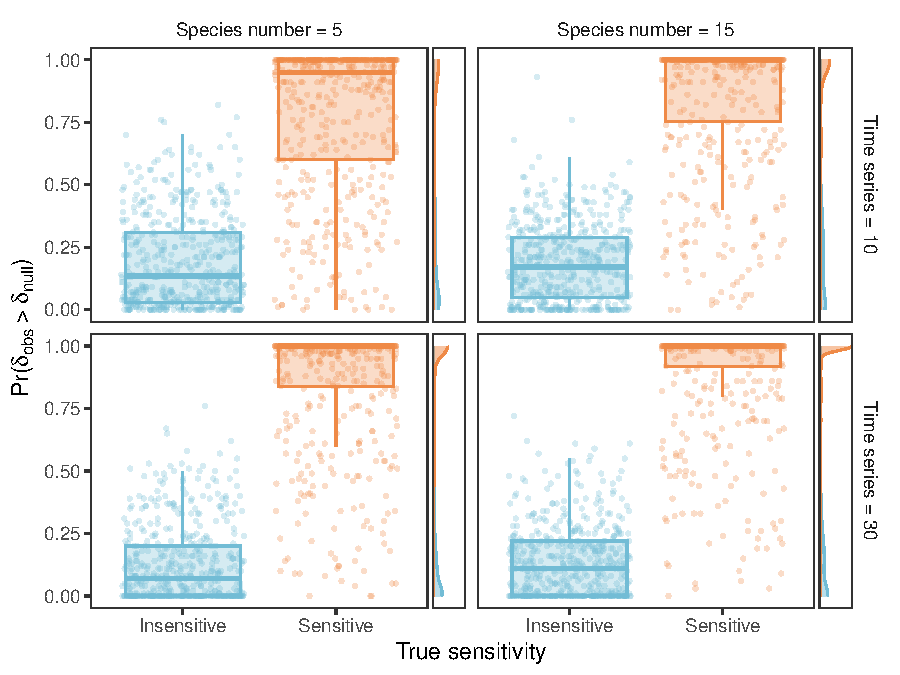
\includegraphics[scale=0.75]{output/figure_eigen.pdf}
    \caption{The proposed method captures the sensitivity to priority effects. The rows and columns distinguish the number of species and the time series length used to generate simulated data. The sensitivity is determined by the leading eigenvalue $\lambda_{max}$ of the community matrix (i.e., sensitive if $|\lambda_{max}| > 1$).}
    \label{fig:box}
\end{wrapfigure}

Here, we use the leading eigenvalue $\lambda_{max}$ of the community matrix (the Jacobian of Equation \ref{eq:m0}) to determine whether the simulated community is sensitive to priority effects.
When the leading eigenvalue satisfies $|\lambda_{max}| < 1$, the community's equilibrium is locally stable and hence no priority effects.
Otherwise ($|\lambda_{max}| > 1$), the community's equilibrium is locally unstable with the possibility of priority effects.
We acknowledge that the criterion of $|\lambda_{max}| > 1$ is a necessary, not sufficient, condition for a priority effect to emerge; yet, it is reasonable to assume that such communities are highly sensitive to priority effects as the equilibrium condition is locally unstable. 

With this sensitivity criterion, we performed a preliminary analysis of the method's performance. We used the model formula presented in Equation \ref{eq:ricker} (the Ricker model) to produce simulated time series data. We considered 224 parameter combinations, within each of which 25 replicates of time series data were produced ($224 \times 25 = 5600$ runs). Parameter values were chosen to yield a sufficient variation in the leading eigenvalue $|\lambda_{max}|$ (Table \ref{tab:param1}).

The results of the preliminary analysis were promising -- \ul{the estimated statistic $\Pr(\delta_{obs} > \delta_{null})$ clearly segregated the insensitive and sensitive communities} (Figure \ref{fig:box}). It is important to note that (i) the number of species did not affect the performance of the proposed method; (ii) the performance was reasonable with a relatively short time series (t = 10). These results may indicate that our method can be applied to a short time series of a species-rich community. 

\textbf{\textit{Method detail: proposed analysis}} -- 
The preliminary analysis ensured that our method has the potential to unveil the sensitivity to priority effects.
In the proposed activity, we will expand the scope of simulation experiments to increase the credibility of our method in other ecological situations.
To this end, we will extend our analysis in two important ways.

(i) \ul{Alternative theoretical model}: ecological systems can exhibit a diversity of competitive interactions; thus, it is important to consider alternative community models describing competitive community dynamics. 
A Beverton-Holt (BH) model is another model widely used in ecology, describing the temporal dynamics of competitive communities. The BH model is formulated as follows:

\begin{equation}
    \label{eq:bh}
    \ln r_i = \ln f(x_i) = r_{0,i} - \ln(1 + \alpha_i x_i + \sum_j \beta_{ij} x_j)
\end{equation}

While the model formula is different, the BH model shares an important feature with the Ricker model: the linear combination of competitive interaction terms.
Hence, as with a Ricker model, a BH model can be simplified as follows (see Box 1 for approximation):

\begin{equation}
    \label{eq:bhmod}
    \ln r_i \approx r_{0,i} - \ln(1 + \gamma_i x_i + \delta_i x_T) + \varepsilon_i
\end{equation}

This formulation indicates that the statistical inference of the key parameter ($\delta_i$) is possible through the fitting of a non-linear model.

(ii) \ul{Broader parameter space}: we will expand the parameter space of the simulation experiment.
Although our preliminary analysis yielded promising results, the parameter space explored is narrow.
By expanding the parameter space for our simulation experiment,  we will confirm the applicability of our method in broader ecological scenarios (Table \ref{tab:param1}).
We will apply this broader parameter space to Ricker and BH models to validate the performance of the proposed method.

Collectively, these proposed activities will increase the credibility of our proposed method.

\begin{table}
    \flushleft
    \caption{Possible parameter values in the proposed and preliminary analysis. In the proposed analysis, we will repeat the analysis across Ricker and Beverton-Holt models to simulate community dynamics.}
    \begin{tabular}{clll}
        Symbol           & Interpretation               & Value (proposed)                                 & Value (preliminary)\\
        \hline
        $r_i$            & Intrinsic population growth  & $\mbox{Unif(\mu_r - h_r, \mu_r + h_r)}$          & \\
        $\mu_r$          & Average $r_i$                & $0.50~\mbox{to}~1.50$                              & 1.00\\
        $h_r$            & Half range in $r_i$          & $0.10~\mbox{to}~0.50$                               & 0.00, 0.10\\  
        $\alpha_{i}$     & Intraspecific competition    & $0.01~\mbox{to}~0.10$                         & 0.01, 0.05\\
        $\beta_{ij}$     & Interspecific competition    & $\mbox{Normal}(\mu_{\beta}, \sigma_{\beta}^2)$   & \\
        $\mu_{\beta}$    & Average interspecific competition & $\alpha_i \times 0.00~\mbox{to}~2.00$ & $0.00~\mbox{to}~1.50$\\
        $\sigma_{\beta}$ & SD interspecific competition & $\mu_{\beta} \times 0.00~\mbox{to}~0.50$ & 0.00, 0.25\\
        $S$              & Number of species in a community & $2, 8, 32, 128$ & 5, 15\\
        $L_t$            & Length of time series            & $5, 10, 20, 40$ & 10, 30\\
        \hline
    \end{tabular}
    \label{tab:param1}
\end{table}

\begin{tcolorbox}[{
  breakable,
  colback=white,
  colframe=gray,
  coltext=black,
  parbox=false,
  boxsep=5pt,
  arc=1pt}]
    Box 1: Approximation of the Beverton-Holt model
    \hline
    In the Beverton-Holt (BH) model, the competition terms are modeled in a logarithmic scale as $\ln(1 + \alpha_i x_i + \sum_j \beta_{ij} x_j)$ (Equation \ref{eq:bh}).
    After the transformation outlined in the maintext, this formula takes the following form $\ln(1 + \gamma_i x_i + \delta_i x_T + e_i)$.
    Here, to separate the nuisance term $e_i$ as an additive term in an ordinary scale, let us denote $c = 1 + \gamma_i x_i + \delta_i x_T$ and consider the Taylor series of $g(e_i) = \ln(c + e_i)$ around $e_i = 0$:

    \begin{equation}
        \label{eq:bhtaylor}
        g(e_i) = \ln(c) + \frac{e_i}{c} - \frac{e_i^2}{2 c^2} + O(e_i),
    \end{equation}

    where $O(e_i)$ denotes the higher-order terms of the Taylor series. If $c \gg 1$ (very likely in empirical data), the higher-order terms may be ignored as $g(e_i) \approx \ln(c) + e_i / c$.
    As a result, after accounting for environmental noise, the BH model can be approximated as:

    \begin{align}
    \begin{split}
        \ln r_i &= r_{0,i} - \ln(1 + \alpha_i x_i + \sum_j \beta_{ij} x_j)\\
                &= r_{0,i} - \ln(1 + \gamma_i x_i + \delta_{i} x_T + e_i)\\
                &\approx r_{0,i} - \ln(1 + \gamma_i x_i + \delta_i x_T) + \varepsilon_i.
    \end{split}
    \end{align}

    This form allows us to estimate the key parameter $\delta_i$ through simple statistical inference.
\end{tcolorbox}

\subsection*{Specific Aim 2: Experimental Validation}

\textbf{\textit{Goal}} -- 
\ul{The overarching goal of this specific aim is to assess the performance of the proposed method using real experimental data, in which the colonization history is experimentally manipulated}.
While simulation experiments provide a strong test case for the model performance, empirical validation is still desired.
We will use published time-series data of microbial communities for the model validation.

\textit{\textbf{Method details: data source}} --
We identified XXX papers that controlled the colonization history of microbes to determine the influence of priority effects (Table XXX).
These data are ideal for our model validation for two reasons. First, the results indicate that several species combinations show a strong sign of priority effects while other combinations do not.
Therefore, we can assess whether the proposed statistic $\Pr(\delta_{obs} > \delta_{null})$ identifies communities in which priority effects manifest.
Second, these experiments vary in time series length and the number of species, allowing us to evaluate the sensitivity of our method to the varied data quality.

\textit{\textbf{Method details: proposed analysis}} --
Our empirical data analysis will proceed as follows:

\begin{enumerate}
    \item Select the appropriate ecological model.
    We will fit Ricker and BH models to an empirical time series and estimate AIC values for each model.
    In the following analysis, we will the model assumption that yields a lower AIC value.
    \item Perform the null model analysis to yield the test statistic $\Pr(\delta_{obs} > \delta_{null})$.
    Note that the model is provided with only time series data (the information on colonization history is not given as data).
    \item Validate the relationship between the community sensitivity to priority effects (known as the experiment outcome) and the test statistic $\Pr(\delta_{obs} > \delta_{null})$.
\end{enumerate}

\subsection*{Specific Aim 3: Application to Field Data}

\end{document}
